\subsection{Front End Schema}

\subsubsection{2*n regular mesh}
Considering the $2*n $ regular mesh Fig .\ref{210f} and the data injection position on the corner.

The speedup vs the number of cores relationship Fig.\ref{corner2n} and Fig.\ref{corner2n2} as follows:

\vspace*{15pt}
\begin{itemize}
\item we can see as the number of cores grows and the equal computational grow as well. 
\item At the same, the $\sigma$ value plays an import role, especially $\sigma > 0.25$. The speedup drops dramatically.
\end{itemize}


\begin{figure}[h]
\centering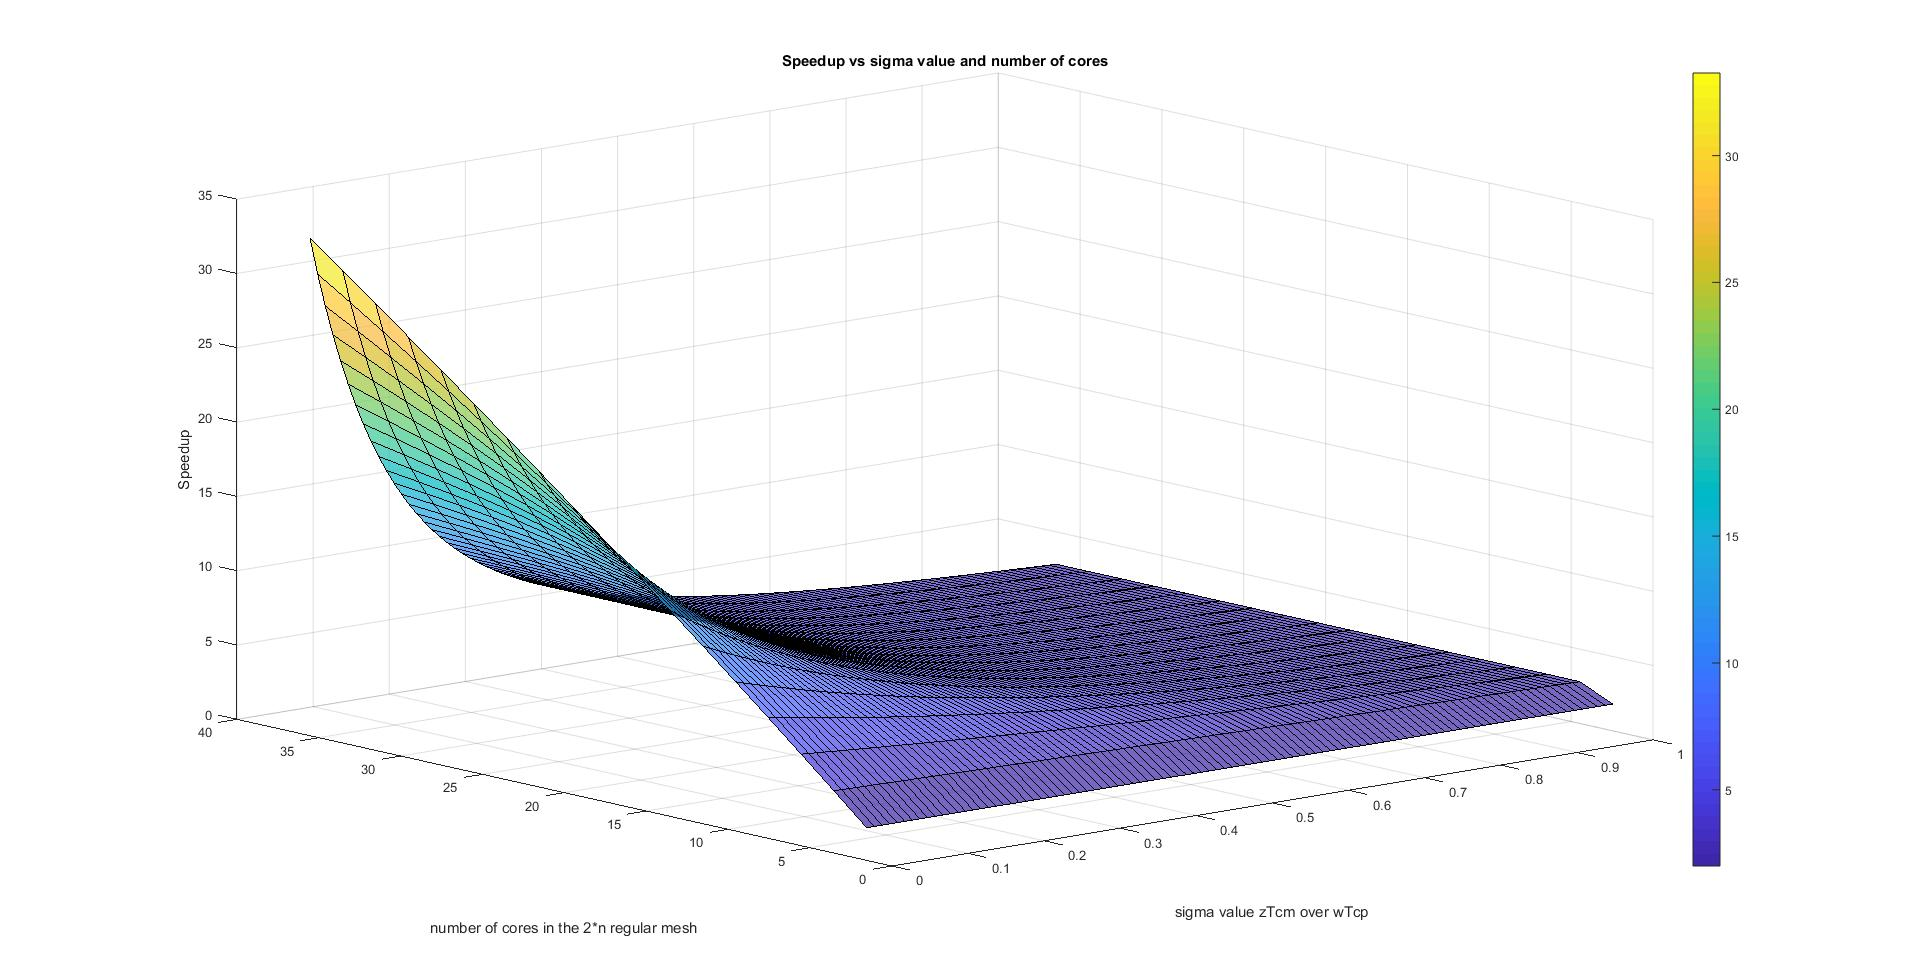
\includegraphics[width=0.85\linewidth]{figure/corner2n}
\caption{Speedup vs $\sigma$ value and number of cores in 2*n regular mesh}
\label{corner2n}
\end{figure}
\vspace*{30pt}

\begin{figure}[h]
\centering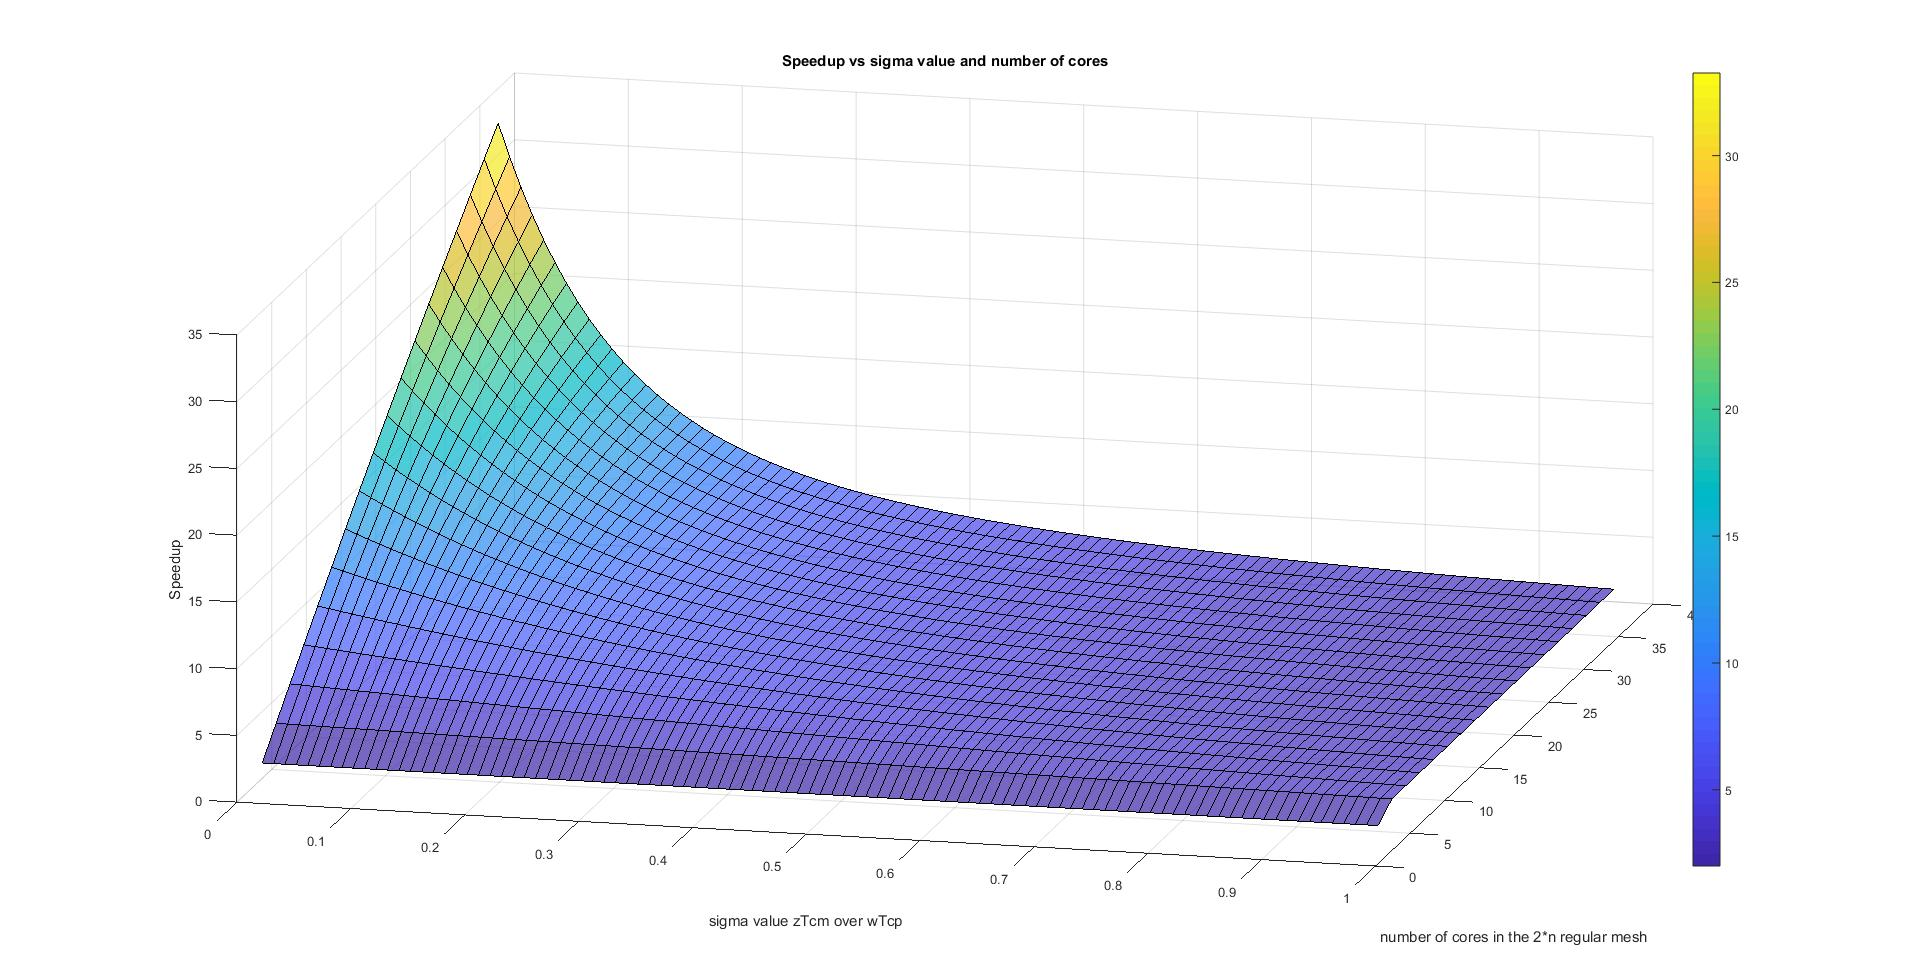
\includegraphics[width=0.85\linewidth]{figure/corner2n2}
\caption{Speedup vs $\sigma$ value and number of cores in 2*n regular mesh}
\label{corner2n2}
\end{figure}


\vspace*{30pt}

\subsubsection{3*n regular mesh simulation result}

Considering the $3*n $ regular mesh Fig .\ref{38f} Fig.\ref{bc3n},which represents the speedup vs the number of cores relationship as follows  Fig.\ref{corner3n}:

\begin{figure}[h]
\centering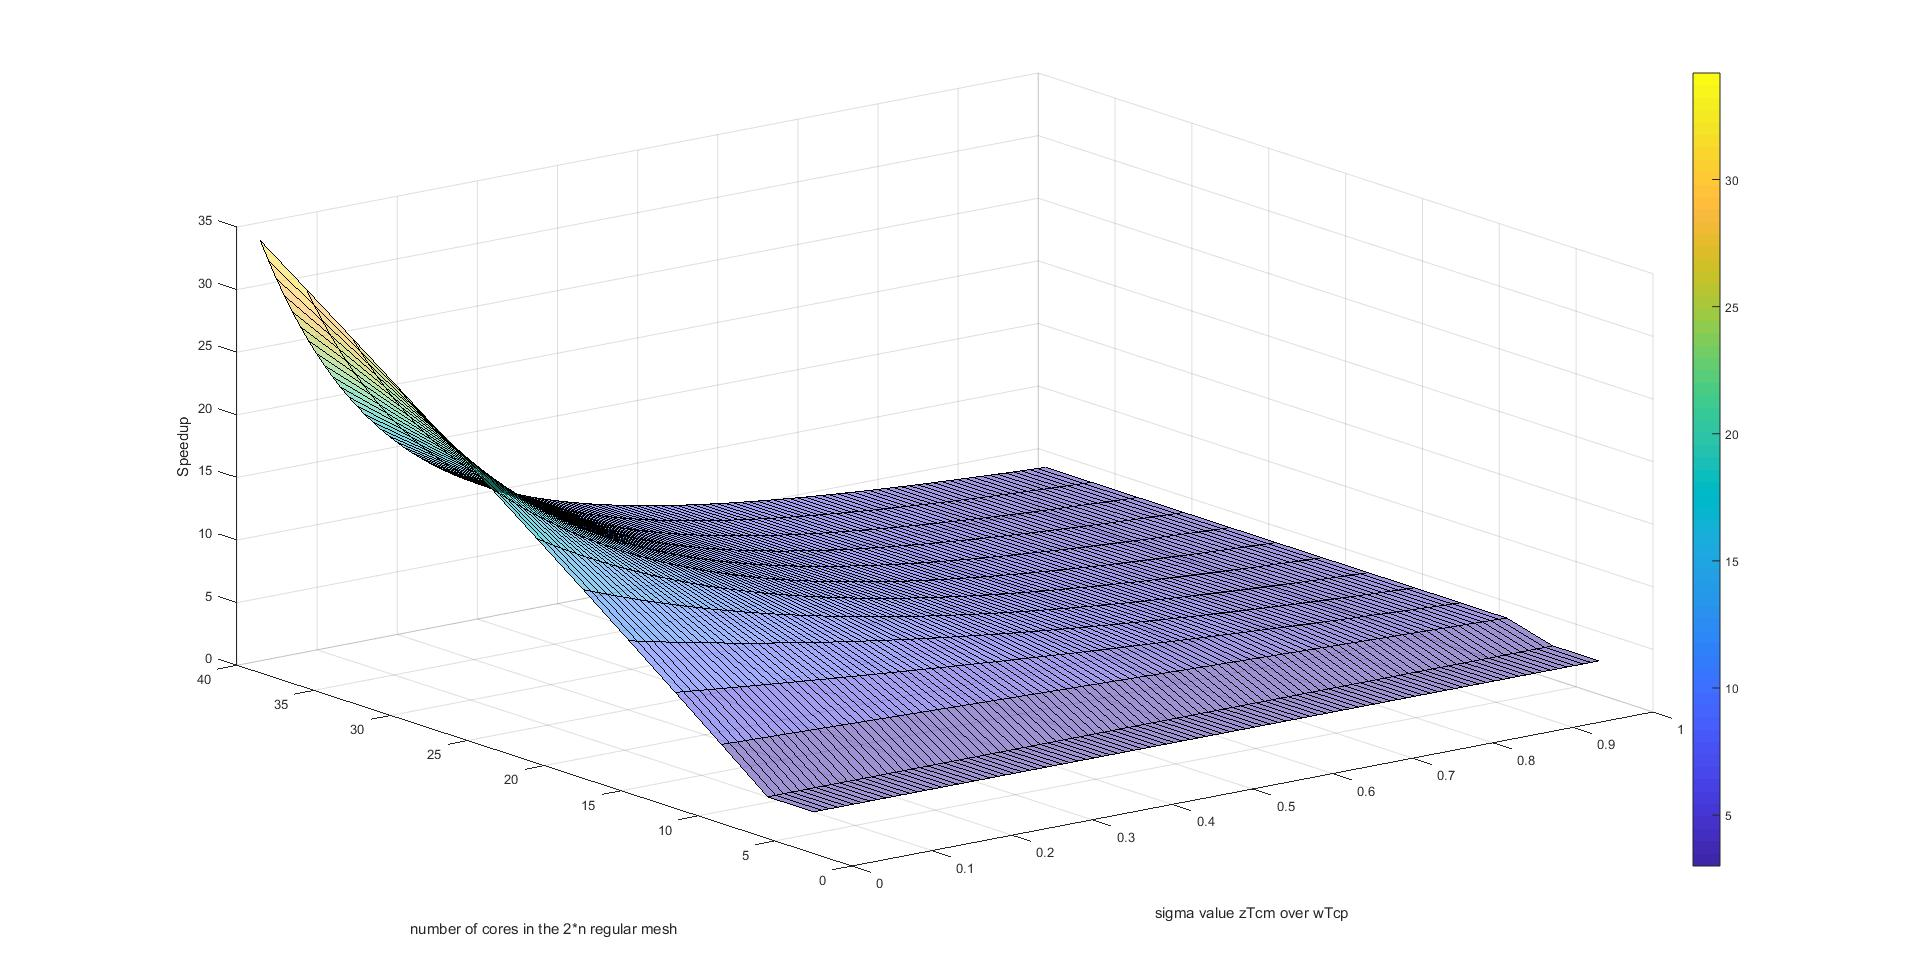
\includegraphics[width=0.85\linewidth]{figure/corner3n}
\caption{Speedup vs $\sigma$ value and number of cores in 3*n regular mesh}
\label{corner3n}
\end{figure}

\vspace*{50pt}

We can see from Fig.\ref{bc3n}. 

\begin{itemize}
\item If the $\sigma > 0.15$, the boundary data injection plan has positive speedup effect comparing with the corner injection plan. 
\item If the $\sigma <= 0.15$, the corner data injection plan will play a more helpful role.
\end{itemize}

\begin{figure}[h]
\centering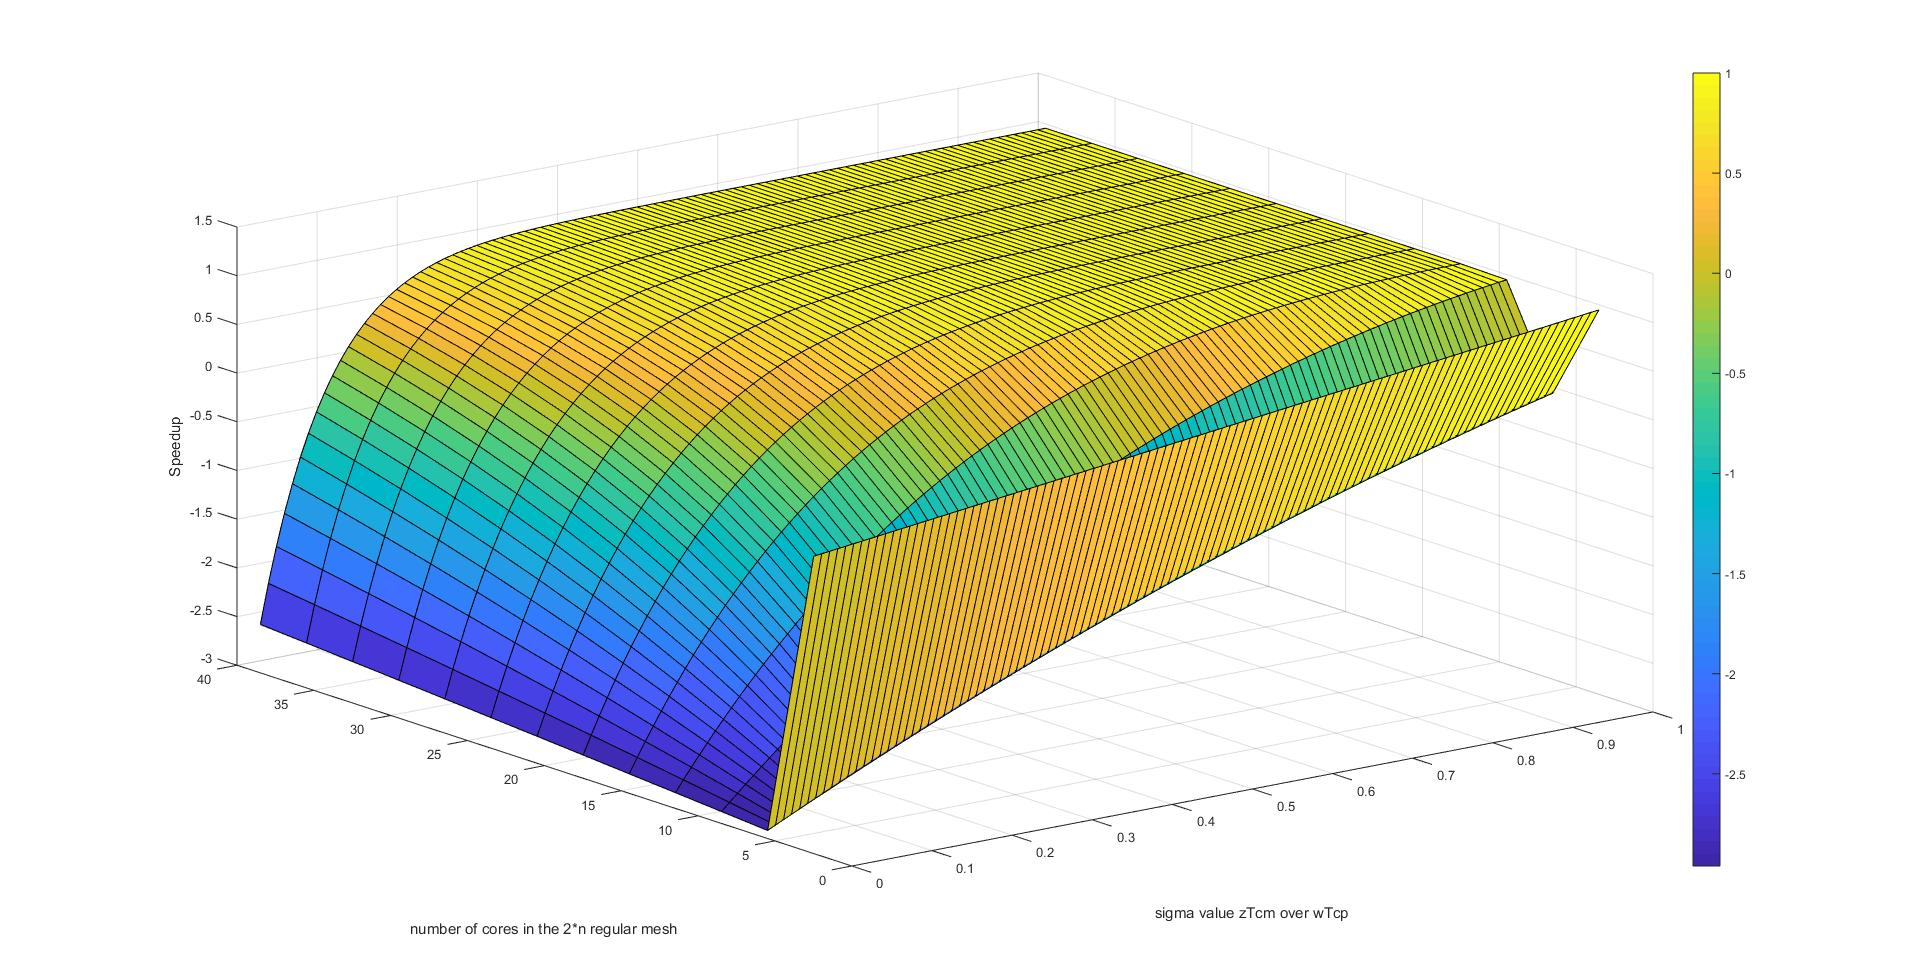
\includegraphics[width=0.85\linewidth]{figure/bc3n}
\caption{Speedup Difference between Corner and Boundary Data Injection in 3*n regular mesh}
\label{bc3n}
\end{figure}

\subsubsection{5*5 regular mesh inner grid simulation result}

Considering the $5*5$ regular mesh Fig .\ref{410f},which represents the speedup vs the number of cores relationship as follows:

The simulation result as follows Fig.\ref{inner4n}:

\begin{figure}[h]
\centering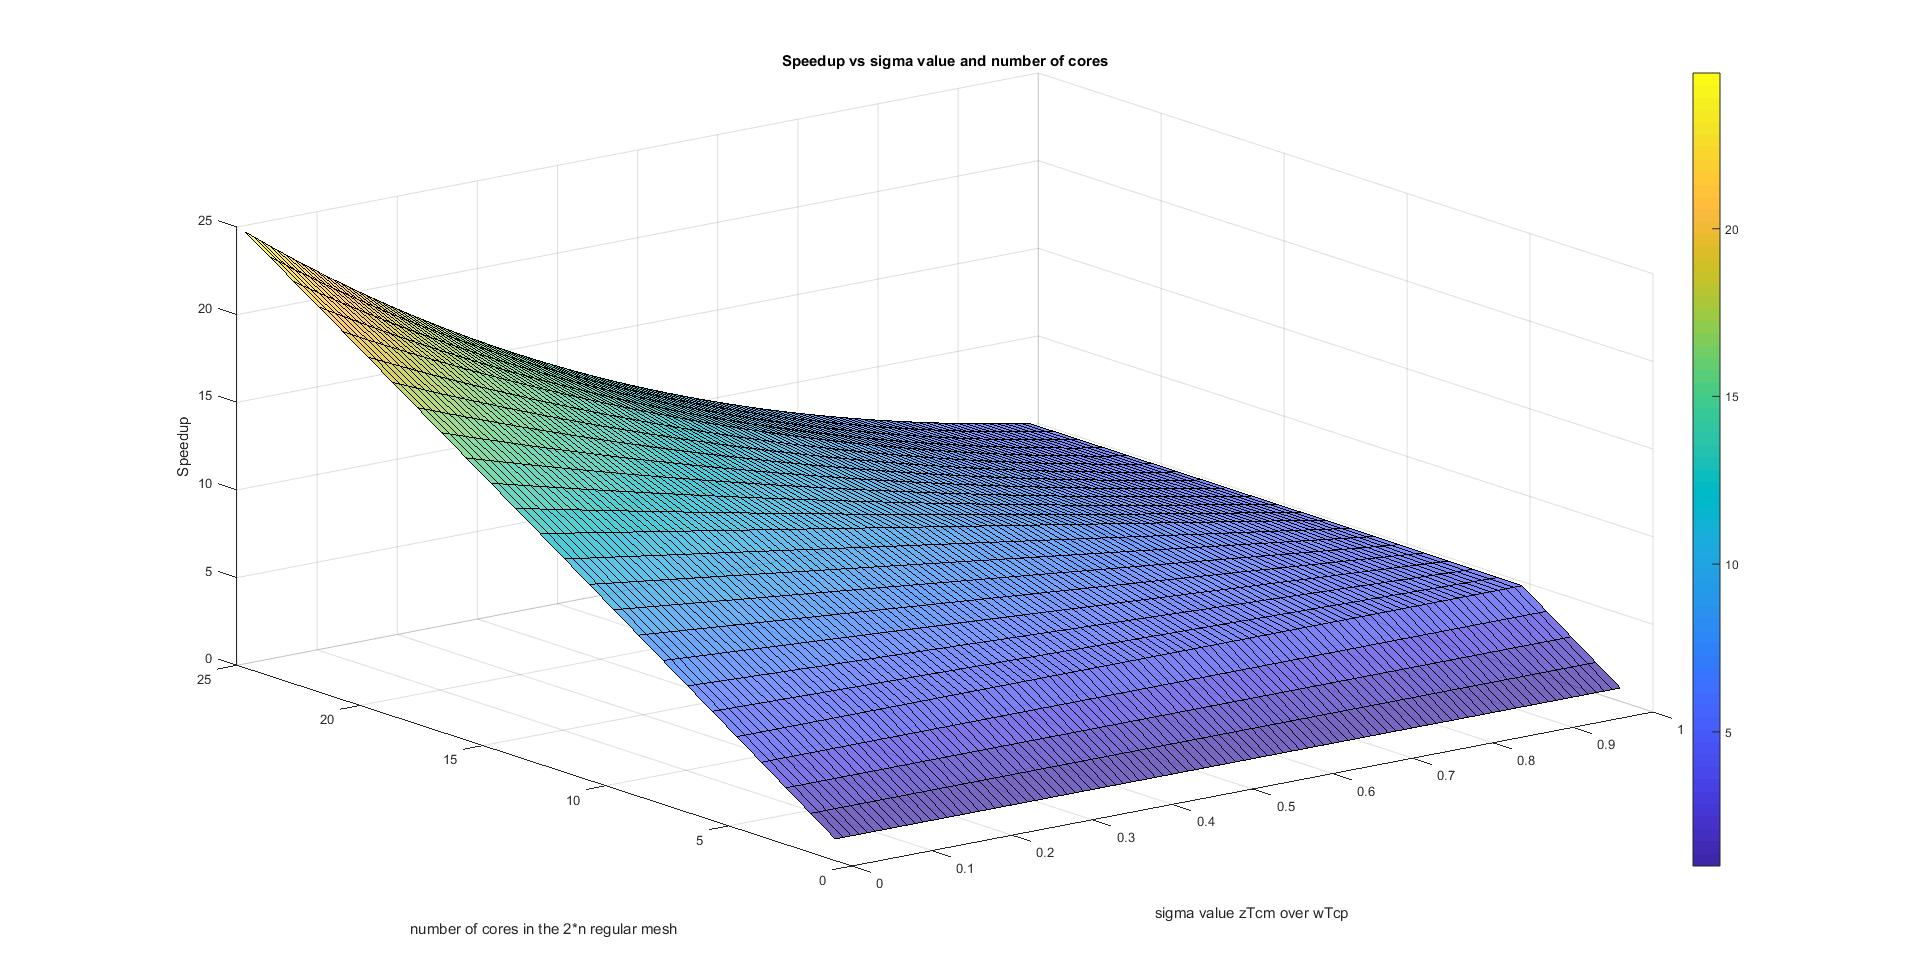
\includegraphics[width=0.85\linewidth]{figure/inner4n}
\caption{Speedup vs $\sigma$ value and number of cores in 4*n regular mesh}
\label{inner4n}
\end{figure}



